\chapter{OSGi-Grundlagen und Softwareverteilung}


Gerade im \ac{IoT}-Umfeld hat sich \ac{OSGi} als eine der Kerntechnologien durchgesetzt.
\glqq Unternehmen wie Cisco, Devolo, Eaton, Miele und Schneider Electric setzen \ac{OSGi} zum Teil schon seit vielen Jahren ein.\grqq\ \cite{osgi_iot_und_mobile}
Auch Bosch setzt im Bereich Smart-Home auf diese Technologie. In einer Umfrage mit etwa 300 Teilnehmern im Jahr 2011 auf der deutschen Java Konferenz JAX in Mainz wurde \ac{OSGi} mit 46\% 
vor RFID/NFC mit 33\% und NoSQL mit 28\% als Kerntechnologie für das Internet der Dinge gewählt \cite{bosch_osgi}. Das vollständige Ergebnis der Umfrage
ist in \autoref{fig:bosch_poll} zu sehen.

\begin{figure}[bh]
 \centering
 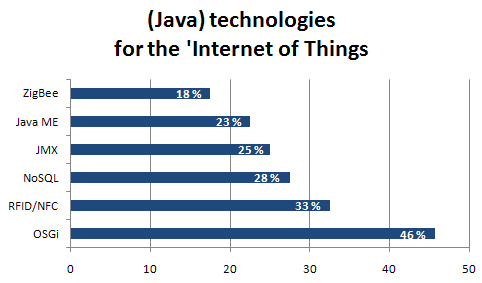
\includegraphics[scale=0.55]{content/pictures/bosch_iot_poll.png}
 % bosch_iot_poll.png: 0x0 pixel, 300dpi, 0.00x0.00 cm, bb=
 \caption{Essential Technologies for the Internet of Things \cite{bosch_osgi}}
 \label{fig:bosch_poll}
\end{figure}

\glqq Firmen wie Cisco gehen im Industriebereich IoT von über 50 Milliarden internetfähigen Geräten bis 2020 und,
abhängig von der Definition, von bedeutend mehr internetfähigen Geräten ab 2020 aus.\grqq\ \cite{osgi_iot_und_mobile}
Eine Vorhersage der IHS Markit geht von mehr als 30 Milliarden IoT-Geräten im Jahre 2020 und einem rasanten Wachstum auf über 75 Milliarden verbundene Geräte im Jahre 2025 aus \cite{ihs_iot_devices}.
Das bedeutet, es existiert eine sehr große Anzahl an Geräten, die direkt oder über Gateways mit dem Internet verbunden und damit angreifbar sind.
Zum Vergleich, Gartner geht im Jahre 2017 von 1,4 Milliarden PCs weltweit aus, Tendenz sinkend \cite{gartner_pcs}. 
Es wird damit voraussichtlich in weniger als drei Jahren mehr als 22-mal so viele \ac{IoT}-Geräte (Things) wie PCs weltweit geben und damit 22-mal mehr potenzielle Angriffsziele für Hacker 
und Cyber-Kriminalität.
Angriffe durch Ransomware wie WannaCry im Mai 2017 oder Petya im Juni 2017 haben aufgezeigt, wie schlecht es um die Sicherheit bei vielen Regierungsinstitutionen, Unternehmen
und Einrichtungen wie Krankenhäusern steht. Die Tatsache, dass einige Betreiber Sicherheitsupdates für ihre Hard- und Software nicht oder nur verspätet einspielen, ist nur schwer zu ändern.
Gerade im \ac{IoT}-Bereich oder bei Smartphones ist es häufiger der Fall, dass die Produktlebensdauer deutlich länger ausfällt, als die Zeitspanne in der Sicherheitsupdates geliefert werden.
So erhält man für das im Oktober 2016 erschienene Pixel Smartphone von Google bereits ab Oktober 2018 keine neue Android Version
und ab Oktober 2019 auch keine Sicherheitsupdates mehr \cite{heise_google_updates}. 
Andere Hersteller bieten zum Teil keine oder nur sehr verzögert Updates an.
Auch aus diesem Grund fordert der Telekom-Chef Tim Höttges eine gesetzliche Verpflichtung zur Bereitstellung von Sicherheitsupdates von Hard- und Softwareherstellern \cite{faz_telekom}.
Die Bereitstellung und Verteilung von Software- und Sicherheitsupdates ist, gerade im Hinblick auf das enorme Wachstum von Things, von enormer Bedeutung.
Mit den einzelnen Themenschwerpunkten Softwareverteilung, \ac{OSGi} und Sicherheit bei der Verteilung von Software, beschäftigen sich viele wissenschaftliche Publikationen.
Es gibt allerdings nur wenige Veröffentlichungen, die gezielt die Forschungsfrage untersuchen, wie eine sichere Verteilung von Softwarekomponenten im Umfeld von \ac{OSGi}
gewährleistet werden kann.\\

Im Folgenden wird auf die für diese Arbeit genutzten wissenschaftlichen Veröffentlichungen eingegangen und die zugrunde liegende Fachliteratur vorgestellt.

\section{Verwandte Arbeiten}

Eine der Grundlagen dieser Arbeit bildet die aktuellste \ac{OSGi}-Spezifikation R6.
Im Mittelpunkt dieser Arbeit stehen die Spezifikationen \ac{OSGi}-Core \cite{osgi_r6} und \ac{OSGi}-Compendium \cite{osgi_r6_compendium}. % die für diese Arbeit benötigten Grundlagen.
Die \ac{OSGi}-Core-Spezifikation enthält Informationen zum Aufbau der \ac{OSGi}-Plattform und bietet Einblicke in den Bundle-Lifecycle, der einen Teil des Softwareverteilungsprozesses ausmacht.
Im \ac{OSGi}-Compendium werden verschiedene Dienste und Komponenten der Plattform beschrieben,
die für die Integration eines Werkzeuges zur Softwareverteilung und für die Empfehlungen zur Weiterentwicklung von Bedeutung sind.\\

Arcangeli et al. \cite{sw_dist} entwickeln in ihrer Arbeit eine moderne Terminologie und Definition für die Softwareverteilung von verteilten Softwaresystemen.
Der von den Autoren beschriebene generische Prozess zur Softwareverteilung dient als Grundlage für den, in dieser Arbeit, entwickelten Prozess 
zur Verteilung von Softwarekomponenten für das OpenMUC-Framework.\\

Die Arbeit von Pursche et al. \cite{osgi_iot_und_mobile} liefert einen Überblick über die Verwendung von \ac{OSGi} im Internet der Dinge und im Bereich des Mobile-Computing.
Neben der Vermittlung der Grundlagen von \ac{OSGi}, werden erfolgreiche Beispiele für den Einsatz von \ac{OSGi} in unterschiedlichen Softwareprojekten vorgestellt.
Das ermöglicht einen einfachen und praxisnahen Zugang zu der behandelten Materie.\\

Weber et al. \cite{osgi_praktiker} behandeln in ihrem Fachbuch verschiedene Komponenten der \ac{OSGi}-Plattform.
Die Arbeit liefert zur \ac{OSGi}-Spezifikation ergänzende Informationen zum Aufbau der Plattform und zu verschiedenen Komponenten wie dem Bundle-Lifecycle.
Des Weiteren beinhaltet die Arbeit Details zur Erstellung von Bundles und \ac{OSGi}-Diensten, die zur Implementierung der Routinen für das Smart-Home-Labor genutzt werden.\\

Weiterführende Informationen zu den Themen Management der \ac{OSGi}-Plattform, Paketierung von Bundles und der Verteilung von Bundles, liefert die Arbeit von Wütherich et al. \cite{osgi_service_platform}.
Diese Informationen dienen in erste Linie der Erarbeitung des Grundlagenkapitels der vorliegenden Arbeit.\\

Die Einschätzung der Sicherheitsaspekte basiert auf der Grundlage der folgenden vier Arbeiten:
(1) Lim et al. \cite{bundle_auth} untersuchen in ihrer Arbeit den Einsatz von Signaturen zum Schutz der Bundles vor Kompromittierung. 
(2) Die Arbeit von Parrend et al. \cite{sfelix} untersucht ebenfalls den Einsatz von Signaturen. Des Weiteren wird
ein alternativer Ansatz vorgestellt, der die sichere Verteilung von Bundles bei geringerem Aufwand ermöglicht.
(3) Hossain et al. \cite{iot_security_issues} beschreiben in ihrer Arbeit verschiedene Sicherheitsprobleme und Herausforderungen im \ac{IoT}-Umfeld.
Für die Sicherheitsbetrachtung der vorliegenden Arbeit sind vor allem die beschriebenen Angriffe auf die Kommunikationskanäle von Gateways und die Kompromittierung von Software relevant.
(4) Die Arbeit von Conti et al. \cite{man_middle} vermittelt eine umfangreiche Übersicht über gängige \ac{MITM}-Angriffe und die Maßnahmen, die zum Schutz ergriffen werden können.\\

Cruz et al. \cite{evaluation_criteria} beschreiben in ihrer Arbeit mehre Szenarien für den Einsatz von Open-Source-Software.
Es werden mehrere Kriterien definiert, die zur Erfüllung der Anforderungen der unterschiedlichen Szenarien beitragen.
Teile der von den Autoren definierten Kriterien finden sich im Kriterienkatalog dieser Arbeit wieder.

\section{Die OSGi-Plattform}
\label{osgi_grundlagen}
Ziel der \ac{OSGi}-Alliance ist es, ein offenes Framework zu definieren, das von einer Vielzahl von Anbietern aus den unterschiedlichsten Bereichen, auf 
einer großen Anzahl von Zielplattformen betrieben werden kann \cite[S. 9]{osgi_r6}.
Dass dieses Ziel erreicht wurde, zeigt sich am vielfältigen Einsatz von \ac{OSGi} in verschiedensten Software-Bereichen.
So gibt es neben Gateways wie ProSyst\footnote{Projektwebseite ProSyst: \url{https://www.bosch-si.com/de/iot-plattform/iot-plattform/gateway/software.html}}
von Bosch und OpenMUC, Implementierungen von Cloud-Plattformen wie z.B. Amdatu\footnote{Projektwebseite Amdatu: \url{https://amdatu.org/}} und eine Vielzahl von Anwendungssoftware, 
die auf \ac{OSGi} basiert. Darunter zum Beispiel auch die sehr beliebten integrierten Entwicklungsumgebungen (\acsu{IDE}) Eclipse\footnote{Projektwebseite Eclipse: \url{http://www.eclipse.org/}}
und IntelliJ\footnote{Projektwebseite IntelliJ: \url{https://www.jetbrains.com/idea/}}.
Vor allem auch im Bereich der Webtechnologien haben sich Projekte und Technologien rund um das Framework gebildet.
So existiert mit Eclipse Virgo\footnote{Projektwebseite Eclipse Virgo: \url{http://www.eclipse.org/virgo/}}, ehemals SpringSource dm Server,
ein modularer und sehr dynamischer Application-Server, der Java Web-, Java Enterprise, Spring-, \ac{OSGi}- und WAR-Applikationen unterstützt und vollständig auf \ac{OSGi} basiert.
Die einzelnen Funktionen des Frameworks sind in verschiedenen Schichten organisiert. 

\subsection{Schichten des Frameworks}
Diese Schichtenarchitektur bildet die Grundlage dafür, dass das \ac{OSGi} Framework so weitreichend eingesetzt werden kann und auch eingesetzt wird.
Im Folgenden werden die Schichten, die in \cite{osgi_r6} spezifiziert sind und in \autoref{fig:osgi_layers} aufgezeigt werden, kurz erläutert.

\begin{figure}[ht]
 \centering
 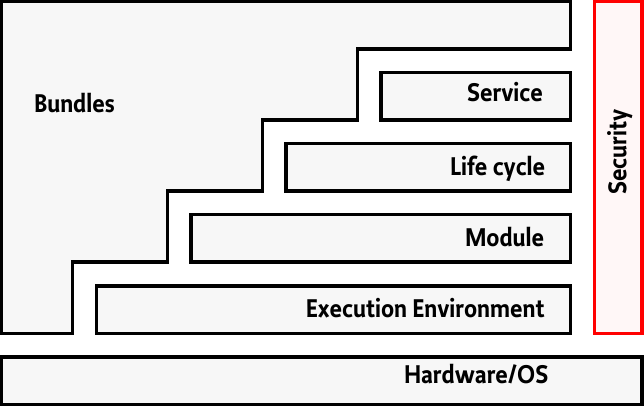
\includegraphics[scale=0.55]{content/pictures/osgi_layers.png}
 \caption{OSGi Core Release 6: Layering \cite[S. 10]{osgi_r6}}
 \label{fig:osgi_layers}
\end{figure}

\begin{description}
 \item [Hardware/OS Layer:]
 Diese Schicht entspricht der Zielplattform auf dem das Framework ausgeführt wird. Als Hardware kann alles eingesetzt werden,  
 vorausgesetzt ein Java-Environment ist auf der Hardware lauffähig. Von einem normalen PC, über eine Set-Top-Box, bis hin zu einem Thing.
 
 \item [Security Layer {\normalfont \cite[S. 17-29]{osgi_r6}}:]
 Diese Schicht wurde im Vergleich zu \ac{OSGi}-Release 1 deutlich erweitert und ist optional. 
 Sie basiert auf dem Sicherheitsmodell der Java 2 Plattform.\footnote{Sicherheitsspezifikation Java 7: \url{http://docs.oracle.com/javase/7/docs/technotes/guides/security/spec/security-spec.doc.html}}
 Mittlerweile ist es möglich, die Authentizität von Code durch das Framework verifizieren zu lassen, z.B. über digital signierte \ac{JAR}-Dateien \cite{osgi_service_platform}. 
 Diese Schicht zieht sich durch alle anderen Schichten, ausgenommen der Hardware/OS-Schicht.
 
 \item[Execution Environment {\normalfont \cite[S. 44-46]{osgi_r6}}:]
 Es gibt verschiedene Java Laufzeitumgebungen, die zum Teil sehr unterschiedliche Module und 
 Klassen innerhalb des java.* Namensraums anbieten. Über das \ac{OSGi}-Execution-Environment werden Bundles über die verfügbaren Laufzeitumgebungen und ihre Fähigkeiten informiert.
 Es gibt die Möglichkeit, eine oder mehrere Laufzeitumgebungen für ein Bundle zu definieren. Dadurch wird verhindert, dass ein Bundle innerhalb eines Execution-Environment gestartet wird, 
 das nicht die nötigen Voraussetzungen im java.* Namensraum bietet.
 
 \item [Module Layer {\normalfont \cite[S. 31-92]{osgi_r6}}:]
 Die Java-Plattform unterliegt in den Bereichen der Paketierung, der Verteilung und Validierung von Java-basierenden Anwendungen und Komponenten
 einer starken Limitierung. Um dieser Limitierung entgegenzuwirken, bietet das \ac{OSGi}-Framework eine standardisierte und generische Lösung zur Modularisierung von Java.
 Diese Limitierung wurde mittlerweile auch von Oracle erkannt und soll mit dem Relase von Java 9 durch das neue \ac{JPMS}-Feature,
 auch bekannt als Jigsaw, verbessert werden \cite{heise_java9}. Ursprünglich war das Release von Java 9 auf den 27. Juli 2017 terminiert, wurde aber im Rahmen des
 Public-Review-Ballot abgelehnt.\footnote{Java-Community-Process JSR \#376: \url{https://www.jcp.org/en/jsr/results?id=5959}}
 Nach weiterer Überarbeitung wurde \ac{JPMS} im zweiten Anlauf angenommen 
 und soll am 21. September 2017 erscheinen \cite{heise_jigsaw}.\footnote{Java-Community-Process JSR \#376: \url{https://www.jcp.org/en/jsr/results?id=6016}}\\
 In \ac{OSGi} wird die Modularisierung durch den Einsatz von Bundles erreicht.
 
 \item[Bundles {\normalfont \cite[S. 31-36]{osgi_r6}}:]
 Ein Bundle wird, wie in Java üblich, als \ac{JAR}-Datei zur Verfügung gestellt.
 Informationen zu einem Bundle werden im Manifest, zu finden im \ac{JAR} unter META-INF/MANIFEST.MF, abgelegt. Darüber können z.B.
 Abhängigkeiten zu anderen Bundles, oder die Sichtbarkeit (Berechtigungen) für die im Bundle verfügbaren Klassen und Module festgelegt werden.
 Es können wie in einem \ac{JAR} üblich, weitere Ressourcen, wie Konfigurationsdateien, Zertifikate oder HTML- und CSS-Dateien abgelegt und verfügbar gemacht werden.
 Innerhalb des OSGI-Frameworks sind Bundles die einzigen Entitäten mit denen Java-basierte Applikationen und Dienste bereitgestellt werden können.
 
 \item [Life Cycle Layer {\normalfont \cite[S. 93-125]{osgi_r6}}:]
 Diese Schicht basiert auf der Module-Schicht und der Security-Schicht und bietet eine Schnittstelle (\ac{API}) zur Kontrolle des Frameworks selbst und seiner Bundles.
 Über diese Schicht wird eine standardisierte Möglichkeit zum Starten des Frameworks angeboten, außerdem muss darüber die Möglichkeit gegeben werden, das OSGi-Framework 
 aus der Ferne zu steuern. Die Life-Cycle-Schicht muss eine Schnittstelle für den Bundle-Life-Cycle bereitstellen. Der Bundle-Life-Cycle ist für diese Arbeit von besonderer Bedeutung.
 Aus diesem Grund wird dieses Thema im \autoref{subsec:bundle_lifecycle} eingehend behandelt.
 
 \item [Service Layer {\normalfont \cite[S. 127-143]{osgi_r6}}:]
 Die Service-Schicht definiert ein Programmiermodell, anhand dessen Softwareentwickler Dienste (Services) programmieren und 
 registrieren können.
 Innerhalb der Schicht findet eine Entkopplung der Definition eines Dienstes und der konkreten Implementierungen statt.
 Dabei verfolgt die Schicht, das durch die \ac{GoF} geprägte Entwurfsprinzip:
 \glqq Program to an Interface, not an implementation.\grqq\ \cite{gof} 
 Ein Dienst wird anhand eines Java-Interfaces beschrieben und kann durch ein oder mehrere Klassen implementiert werden.
 Verfügbare Implementierungen können dann zur Laufzeit gesucht, ausgewählt und von den Bundles genutzt werden. 
\end{description}


Diese Schichten bilden den Kern des \ac{OSGi}-Frameworks. Über den Bundle-Lifecycle ist es möglich, weitere Bundles zu installieren, zu aktualisieren und zu entfernen.
Dadurch ist es möglich, das Framework beliebig zu erweitern.

\subsection{Der Bundle-Context und der Bundle-Lifecycle}
\label{subsec:bundle_lifecycle}

Über den Bundle-Context lassen sich neue Bundles in das Framework einbringen und bereits installierte Bundles steuern \cite{osgi_praktiker}.
Der Bundle-Context ist ein Teil der Life-Cycle-Schicht und stellt eine Verbindung zwischen dem Framework und seinen Bundles her.
Über diese Funktionalität wird die Softwareverteilung und das Aktualisieren von Software innerhalb von \ac{OSGi} erst möglich.
Für jedes installierte Bundle existiert ein korrespondierendes Bundle-Objekt. Über dieses Objekt lässt sich der Bundle-Lifecycle steuern. 
Jedes Bundle kann innerhalb des Frameworks über mehrere Attribute identifiziert werden. Bei der Installation bekommt jedes Bundle 
automatisch eine eindeutige ID (Bundle Identifier) zugewiesen. 
Die Attribute-Bundle-Location wird bei der Installation ermittelt und ist in den meisten Fällen die \acsu{URL}, unter welcher die \ac{JAR}-Datei zu finden ist.
Auch dieses Attribut muss innerhalb des Frameworks eindeutig sein.
Außerdem muss jedes Bundle einen symbolischen Namen (Bundle Symbolic Name) und eine Version (Bundle Version) besitzen. 
Diese beiden Attribute müssen in Kombination eindeutig sein, um das Bundle innerhalb des Frameworks identifizieren zu können.
Die Versionsnummer (Bundle Version) wird in \ac{OSGi}, wie bei maven-Paketen\footnote{Maven Softwareprojekt Managementwerkzeug: \url{https://maven.apache.org/}}
auch, nach den Regeln des Semantic-Versioning gebildet\footnote{Webseite der Semantic-Versioning-Spezifikation: \url{http://semver.org/}}\ \cite[S. 54]{osgi_r6}.
Eine Version besteht, wie in \autoref{fig:osgi_versioning} dargestellt, aus den drei Teilen major (1), minor (2), micro(3). Diese werden per Punkt (.) voneinander getrennt.
\begin{figure}[h]
  \centering
  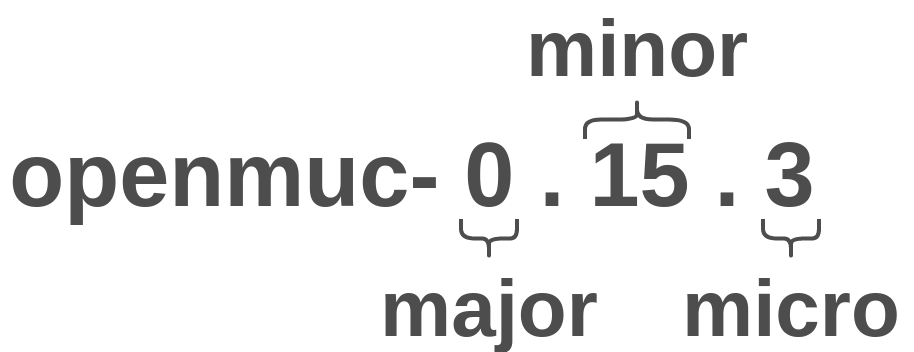
\includegraphics[scale=0.15]{content/pictures/semantic_versioning.png}
  \caption{Aufbau der Versionsnummer nach Semantic-Versioning}
  \label{fig:osgi_versioning}
\end{figure}

\begin{description}
 \item [major:] Repräsentiert den Stand der API. Wird erhöht wenn Änderungen veröffentlicht werden, die inkompatibel zu vorherigen Versionen der API sind.
 \item [minor:] Wird erhöht, wenn eine neue Funktionalität in das Bundle eingepflegt wurde, die kompatibel zur bestehenden API ist.
 \item [micro:] Wird erhöht, wenn durch das Update ein Fehler an bestehender Funktionalität behoben wurde.
\end{description}

Innerhalb des Manifests kann über den Namen und die Versionsnummer eines Bundles, die Abhängigkeit und Anforderungen an das Patchlevel dieses Bundles definiert werden.
OSGi erlaubt es zur Laufzeit neue Bundles in das Framework zu integrieren und bestehende Bundles zu starten, stoppen, aktualisieren und zu entfernen.
Dies geschieht über den Bundle-Lifecycle. Der Lebenszyklus eines Bundles lässt sich, wie in \autoref{fig:bundle_lifecycle} zu sehen, über ein Zustandsdiagramm abbilden.\\

Bevor ein Bundle installiert \textit{(install)} werden kann, wird es validiert. Es existieren mehrere Spezifikationen für unterschiedliche Versionen des Manifests. 
Beinhaltet das Manifest eines Bundles nicht alle in der entsprechenden Spezifikation festgelegten Attribute, oder weist es syntaktische Fehler auf, ist das Bundle ungültig
und kann nicht installiert werden.
Entspricht das Manifest des Bundles den Spezifikationen, wird es im persistenten Speicher des Frameworks abgelegt und geht in den Zustand \textit{INSTALLED} über.\\

Als nächstes wird geprüft \textit{(resolve)}, ob die im Manifest definierten Abhängigkeiten zu anderen Java-Klassen aufgelöst werden können.
Sind alle benötigten Klassen verfügbar, geht das Bundle in den Zustand \textit{RESOLVED} über \cite{osgi_service_platform}.
Nur aus diesem Zustand ist es möglich, das Bundle zu starten \textit{(start)}.
Des Weiteren kann aus diesem Zustand das Bundle deinstalliert \textit{(uninstall)} , aufgefrischt \textit{(refresh)} und aktualisiert \textit{(update)} werden.

\begin{figure}[ht]
 \centering
 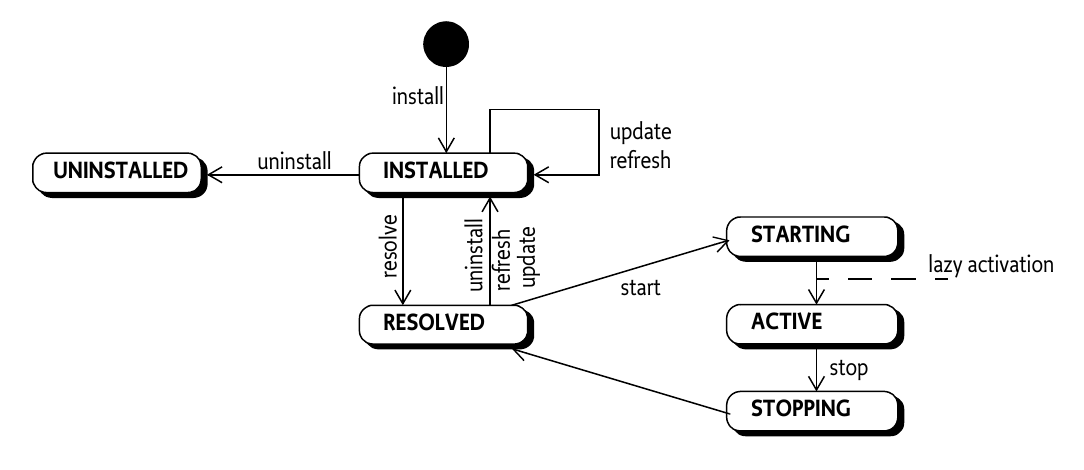
\includegraphics[scale=0.5]{content/pictures/osgi_bundle_lifecycle.png}
 \caption{\ac{OSGi} Core Release 6: State diagram Bundle \cite[S. 107]{osgi_r6}}
 \label{fig:bundle_lifecycle}
\end{figure}

Das Bundle wird gestartet, indem die \textit{start}-Methode des BundleActivator aufgerufen wird. Das Bundle verbleibt im Zustand \textit{STARTING}, solange die \textit{start}-Methode 
nicht beendet wurde. Wird die \textit{start}-Methode ausgeführt, ohne dass ein Fehler (Exception) auftritt, geht das Bundle in den Zustand \textit{ACTIVE} über.
Eine Ausnahme bilden Bundles, bei denen die Richtlinie zur Aktivierung auf lazy eingestellt ist.
In diesem Fall verweilt das Bundle im Zustand \textit{STARTING}, bis die erste Klasse aus dem Bundle geladen werden soll.
Aus dem Zustand \textit{ACTIVE} kann das Bundle gestoppt \textit{(stop)} werden. Es verweilt in dem Zustand \textit{STOPPING}, bis die \textit{stop}-Methode des BundleActivator beendet ist.
Nach Beendigung der \textit{stop}-Methode geht das Bundle wieder in den Zustand \textit{RESOLVED} über.\\

Aus \textit{INSTALLED} und \textit{RESOLVED} kann ein Bundle deinstalliert \textit{(unintall)} werden. Wenn das Bundle nicht durch weitere Bundles in Benutzung ist, wird das Bundle aus 
dem persistenten Speicher des Frameworks entfernt und in den Zustand \textit{UNINSTALLED} überführt. Aus diesem Zustand kann in keinen anderen Zustand mehr gewechselt werden.
Sollte das Bundle in Benutzung sein, bleiben die durch das Bundle zur Verfügung gestellten Klassen und Ressourcen weiter verfügbar, bis das Bundle erneuert \textit{(refresh)} wird 
oder das Framework neu gestartet wird.\\

Im Zustand \textit{RESOLVED} is es im Weiteren möglich, das Bunde zu aktualisieren \textit{(update)} oder zu erneuern \textit{(refresh)}.
Bei einem Update wird ein bestehendes Bundle durch eine neuere Version desselben Bundles ersetzt. Nach dem Update muss sich das Bundle im selben Zustand befinden,
wie zu Beginn der Aktualisierung. Bei einem Update ist das Verhalten, wenn das Bundle in Benutzung ist, dasselbe wie beim Deinstallieren eines Bundles.
Die  Klassen und Ressourcen des alten Bundles bleiben verfügbar, bis das Bundle erneuert wird oder das Framework neu gestartet wird.
Bei einer Erneuerung werden die Abhängigkeiten des Bundles erneut aufgelöst.
Existieren Bundles mit aktiver Abhängigkeit zu diesem erneuerten Bundle, werden diese ebenfalls erneuert.
Das sorgt bei einem Update dafür, dass die Referenzen auf die alten Klassen und Ressourcen aufgegeben werden und durch die Klassen und Ressourcen aus dem Update ersetzt werden.\\

In diesem Abschnitt wurde nur ein Teil der gesamten Funktionalität des \ac{OSGi}-Frame\-works beschrieben.
Dabei handelt es sich um den Teil, der für die Etablierung und Integration eines Softwareverteilungsprozesses unabdingbar ist.


\section{Prozess der Softwareverteilung}
\label{prozess_der_softwareverteilung}
Für den Begriff der Softwareverteilung und dessen Prozess existieren etliche Definitionen, die eine einheitliche Definition
dieses Prozesses und seiner Begrifflichkeiten stark erschweren. 
So beschreibt Dearle \cite{sw_dist_dearle} die Softwareverteilung wie folgt:
Der Prozess der Softwareverteilung findet zwischen dem Erwerb der Software und ihrer Ausführung statt.
Er besteht aus einer Anzahl von Aktivitäten, die in gegenseitiger Beziehung stehen.
Zum Beispiel der Veröffentlichung, der Konfiguration, der Aktualisierung und der Deaktivierung der Software.\\

Eine deutlich differenziertere Definition liefern Arcangeli et al.: 
\glqq We define software deployment as a process which organizes and schedules a set of activities in order
to make software available for use and to keep it up-to-date and operational.\grqq\ \cite{sw_dist}
Die Softwareverteilung umfasst nach dieser Definition nicht nur die Aktivität der Verteilung, sondern auch die 
kontinuierliche Pflege der Software und ihre Deinstallation.
Arcangeli et al. \cite{sw_dist} definieren sechs, für den Prozess maßgebliche Aktivitäten für die Verteilung der Softwarekomponente und drei weitere für den 
Bereich der Instandhaltung.
Den Einfluss der verschiedenen Aktivitäten auf den Zustand der Software kann über ein Zustandsdiagramm, zu sehen in \autoref{fig:sw_deploy_states}, dargestellt werden. \\

\begin{figure}[h]
 \centering
 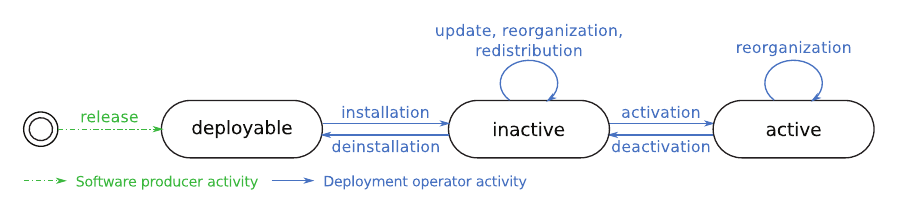
\includegraphics[width=11cm]{content/pictures/sw_deploy_states.png}
 \caption{Impact of the activities on the state of the software. \cite{sw_dist}}
 \label{fig:sw_deploy_states}
\end{figure}

Die Aktivität veröffentlichen \textit{(release)} (1) umfasst die Arbeiten, die nötig sind die Software zu paketieren und für die Verteilung vorzubereiten.
Diese Tätigkeit ist Aufgabe des Herstellers der Softwarekomponente.
Bei der Installation \textit{(installation)} (2) wird die Komponente auf Seiten des Verbrauchers in ein Gesamtsystem eingebettet. Dies umfasst die Verteilung bzw. den Transfer
und die Konfiguration der Softwarekomponente, um sie für die Aktivierung bereit zu machen.
Unter Aktivierung \textit{(activiation)} (3) versteht man alle Operationen, die notwendig sind, um die Software
in das Gesamtsystem zu integrieren und zu betreiben. Diesem Prozess entgegengesetzt ist die Deaktivierung \textit{(deactivation)} (4). Darunter
fallen alle Aufgaben, die notwendig sind, um den Betrieb der Software zu stoppen. Dies beinhaltet auch, die von der Software abhängigen 
Komponenten über die Abschaltung zu informieren. Die Deinstallation \textit{(deinstallation)} (5) sorgt dafür, dass die Softwarekomponente auf Seiten des Verbrauchers
entfernt wird.
Die letzte der sechs maßgeblichen Tätigkeit ist die Außerbetriebnahme \textit{(retire)} (6) der Softwarekomponente.
Diese Tätigkeit findet wieder auf Seiten des Herstellers statt und hat keinen Einfluss auf die bei einem Verbraucher betriebenen Komponenten.
Sie ist demnach kein direkter Teil der Verteilung.\\

Für den Betrieb und die Wartung der Komponente sind drei weitere Wartungsaktivitäten definiert.
Wird durch den Hersteller eine neue Version einer Softwarekomponente veröffentlicht, kann diese per Aktualisierung \textit{(update)} (7) in das System eingebracht werden. Dabei wird die 
veraltete Komponente ersetzt. Weitere Wartungsaktivitäten sind die Reorganisation \textit{(reorganization)} (8) und die Neuverteilung \textit{(redistribution)} (9).
Bei einer Reorganisation wird die logische Struktur des Gesamtsystems verändert, zum Beispiel in dem einzelne Komponenten ersetzt oder zusammengefasst werden.
Bei einer Neuverteilung wird die physische Struktur des Systems verändert. Das ist zum Beispiel dann der Fall, wenn (Teil-)Systeme, oder Komponenten auf eine andere Hardware bewegt werden.\\

Eine Softwarekomponente kann nach Veröffentlichungen oder Deinstallation auf ein Zielsystem installiert werden.
Dadurch wechselt der Zustand von \textit{deployable} zu \textit{inactive}.
In diesem inaktiven Zustand können Wartungsaktivitäten durchgeführt werden oder die Komponente aktiviert werden.
War die Aktivierung erfolgreich, geht die Komponente in den Zustand \textit{active} über. Von dort kann sie 
reorganisiert oder deaktiviert werden.\\

\subsection{Parallelen zum Bundle Lifecycle von OSGi}

Vergleicht man das Zustandsdiagramm aus \autoref{fig:sw_deploy_states} mit dem des Bundle-Lifecycle aus \autoref{fig:bundle_lifecycle}, können einige Überschneidungen festgestellt werden.
Diese sind in \autoref{fig:osgi_deploy_process_1} kenntlich gemacht. So entspricht der Zustand \textit{inactive} einer Zusammenfassung der Zustände \textit{INSTALLED} und \textit{RESOLVED}
aus dem Bundle-Lifecycle.
Der Zustand \textit{active} wiederum umfasst die drei Zustände \textit{STARTING}, \textit{ACTIVE} und \textit{STOPPING} aus \ac{OSGi}.

\begin{figure}[h]
 \centering
 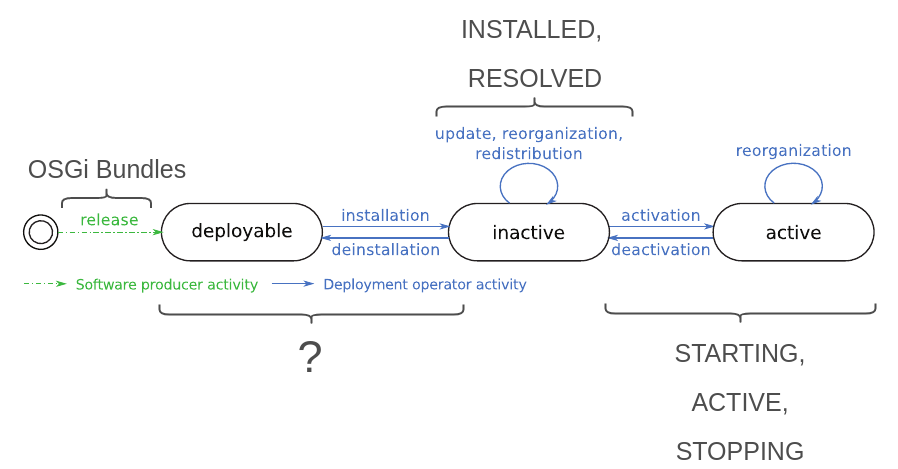
\includegraphics[width=11cm]{../02.Diagramme/osgi_deploy_process_1.png}
 \caption{\ac{OSGi}-Softwareverteilung auf Basis des Prozesses von Arcangeli et al. \cite{sw_dist}}
 \label{fig:osgi_deploy_process_1}
\end{figure}

Das bedeutet, dass ein Teil des Softwareverteilungsprozesses bereits durch das \ac{OSGi}-Framework bereitgestellt wird. 
Zur vollständigen Erfüllung des Prozesses nach Arcangeli et al. \cite{sw_dist} fehlt noch die Paketierung und Verteilung der Komponenten.
Für eine einheitliche Paketierung ist durch die Spezifikation der \ac{OSGi}-Bundles bereits gesorgt. Damit bleibt noch der Punkt der Verteilung der Komponenten übrig.
Dieser letzte Baustein im Prozess der Softwareverteilung für \ac{OSGi}-basierte Anwendungen wird im weiteren Verlauf der Arbeit identifiziert und in 
das OpenMUC-Framework integriert. Bevor dieses Kapitel mit der Vorstellung des OpenMUC-Frameworks geschlossen wird, 
werden einige Sicherheitsaspekte in Bezug auf die Softwareverteilung betrachtet.

\section{Aspekte der Sicherheit}
\label{sicherheit}
Eine vollständige Sicherheitsanalyse von OpenMUC liegt außerhalb der Zielsetzung dieser Arbeit.
An dieser Stelle werden ausschließlich Sicherheitsaspekte erläutert, die später zur Validierung geeigneter Technologien zur Softwareverteilung 
herangezogen werden. Wie in \autoref{prozess_der_softwareverteilung} dargestellt, muss zur Vervollständigung des Softwareverteilungsprozesses
eine Technologie gefunden und in OpenMUC integriert werden, welche die Aufgabe zur Bereitstellung und Verteilung von Bundles übernimmt. \\

Für die folgende Untersuchung der Sicherheitsaspekte wird von einem zentralen Managementsystem ausgegangen. Dieses hält die verfügbaren Bundles vor und 
verteilt diese zum Zweck der Installation und Aktualisierung auf einer OpenMUC Installation, im weiteren Target genannt.
Ausgehend von dieser Architektur können drei Angriffsvektoren identifiziert werden: (1) eine Kompromittierung der Management-Software,
(2) eine Kompromittierung der im Repository verfügbaren Bundles und (3) ein \ac{MITM}-Angriff auf die Verbindung
zwischen Managementsystem und Target.\\

(1) Für die Bereitstellung des oben genannten Managementsystems muss eine weitere Software eingesetzt werden.
Diese kann durch Fehler oder durch falsche Konfigurationen kompromittiert werden.
Je nach Schwere der Kompromittierung könnten Angreifer die volle Kontrolle über die mit dem Managementsystem verbundenen Targets erlangen. 
So weit verfügbar, werden bestehende Untersuchungen zur Sicherheit und die Anzahl und Schwere von bekannten Fehlern der Software in die Bewertung einfließen.\\

(2) Werden bestehende Bundles um Schadcode erweitert oder durch bösartige Bundles ersetzt, können Targets einfach kompromittiert werden.
Zu demselben Schluss kommen Hee-Young et al. in ihrer Arbeit \cite{bundle_auth}. Die Autoren sehen im Verteilen von Bundles 
eine schwerwiegende Möglichkeit, die Sicherheit einer \ac{OSGi}-Installation zu unterwandern.
Auch Parrend et al. \cite{sfelix} sehen im Verteilen von \ac{OSGi}-Bundles eine der größten Herausforderungen in Bezug auf die Sicherheit des Targets.
Über schadhafte Bundles können bestehende Dienste kompromittiert und neue bösartige Dienste in das 
\ac{OSGi}-Framework eingebracht werden. Über diese Dienste können Angreifer weitere Angriffe initiieren und das Target somit unter ihre Kontrolle bringen. 
Wie in \autoref{osgi_grundlagen} beschrieben, gibt es mittlerweile die Möglichkeit, \ac{OSGi}-Bundles zu signieren.
Laut Parrend et al. \cite{sfelix}, hat die im \ac{OSGi}-Framework zum Einsatz kommende Signatur-Methode hohe Anforderungen an die Hardware.
Das steht im Konflikt mit dem Ziel, \ac{OSGi} auf möglichst vielen Plattform einsetzen zu können, da der Einsatz von signierten Bundles ein gewisses Maß an Ressourcen
auf dem Target voraussetzt.
In ihrer Arbeit \cite{sfelix} werden verschiedene Lösungen zur sicheren Authentifizierung mit geringeren Anforderungen an Ressourcen vorgestellt. 
Die Werkzeuge zur Softwareverteilung werden auf die Möglichkeit hin untersucht, eine optimierte Methode zur Signatur von Bundles einzusetzen.\\

(3) Ein beliebtes Angriffsziel bei verteilten Systemen ist der Kommunikationskanal \cite{iot_security_issues}.
Verschafft sich ein Angreifer mittels \ac{MITM}-Angriff Zugang zu der Kommunikation 
zwischen Managementsystem und Target, können Bundles on-the-fly manipuliert oder nicht-autorisierte Steuerbefehle abgesetzt werden.
Conti et al. \cite{man_middle} vermitteln in ihrer Arbeit eine übersichtliche Darstellung gängiger \ac{MITM}-Angriffe.
Laut den Autoren ist diese Art des Angriffs heutzutage eine der größten Sorgen von Sicherheitsexperten. Je nach eingesetzten Kommunikationsprotokollen kommen verschiedene Arten des Angriffes
zum Tragen. Nach Einschätzung von Conti et al. \cite{man_middle} kann ein Schutz vor \ac{MITM}-Angriffen durch eine starke Ende-zu-Ende-Verschlüsselung der Kommunikationsteilnehmer
erreicht werden. Des Weiteren sollten Schlüssel über sichere Kanäle ausgetauscht werden und von einer vertrauenswürdigen Zertifizierungsstelle (\ac{CA}) signiert sein.
Die Ende-zu-Ende-Verschlüsselung ist damit ein weiteres Kriterium für die zu untersuchenden Werkzeuge zur Softwareverteilung.\\

Werden diese drei Aspekte bei der Bewertung der Werkzeuge zur Softwareverteilung berücksichtigt, kann davon ausgegangen werden,
dass die Gefährdung von OpenMUC durch die zusätzliche Komponente auf ein Minimum reduziert ist. Im nun folgenden Abschnitt wird das OpenMUC-Framework eingehend beschrieben.

\section{OpenMUC}
\acs{MUC} steht für \aclu{MUC}. 
\glqq Der Multi Utility Communication-Con\-troller  (MUC-Controller) ist Kern der deutschen Standardisierungsbemühungen  
im Bereich Smart Metering. Er dient als Gateway, das mehrere Energie- und Wasserzähler bündelt und Messwerte konzentriert
auf den Abrufserver hochlädt.\grqq\ \cite{ise_muc}
Bei OpenMUC handelt es sich um ein Energy-Management-Gateway, das man heutzutage der \ac{IoT}-Domäne Smart-Energy zuordnet.\\

Die Aufgabe von OpenMUC besteht darin, die Funktionalität des MUC-Standards zu implementieren und den Standard weiter voranzutreiben.
Außerdem soll ein dynamisches und möglichst generisches Framework geschaffen werden, um heutige und zukünftige Probleme im Bereich der \ac{IoT}-Gateways zu lösen.
Die Architektur von OpenMUC-Frameworks ist in \autoref{fig:openmuc_architecture} zu sehen. 

\begin{figure}[h]
 \centering
 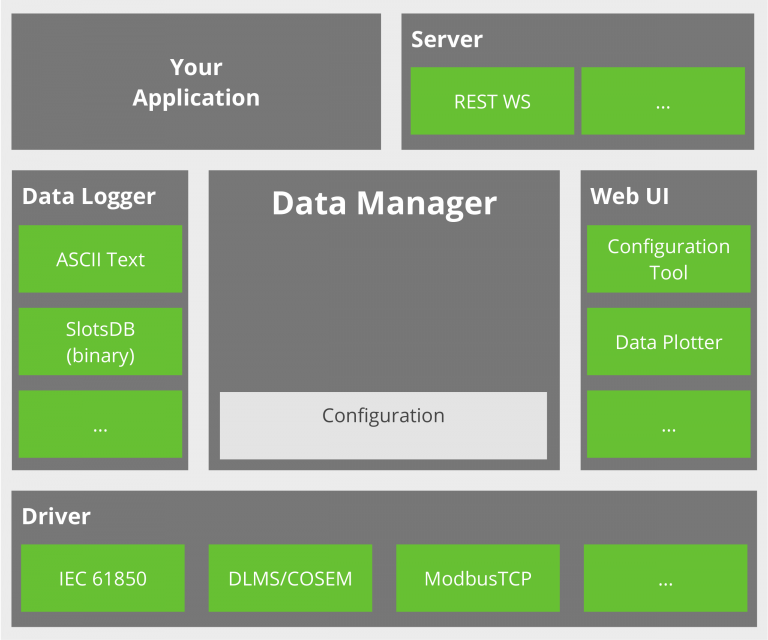
\includegraphics[scale=0.50]{content/pictures/openmuc_architecture.png}
 \caption{OpenMUC Architecture \cite{openmuc}}
 \label{fig:openmuc_architecture}
\end{figure}

Der momentane Einsatzschwerpunkt von OpenMUC liegt im Bereich der intelligenten Energienetze und wird in diesem Bereich hauptsächlich am Fraunhofer-\ac{ISE} und bei der Siemens AG eingesetzt.
Wie diese Arbeit im weiteren Verlauf noch zeigen wird, ist ein Einsatz des Frameworks nicht ausschließlich auf diese Domäne beschränkt.
Zwei Ziele standen bei der Entwicklung besonders im Vordergrund. Zum einen soll OpenMUC möglichst modular sein, um z.B. neue Kommunikationsprotokolle oder Steuermodule einfach
integrieren zu können und so die Funktionalität flexibel zu erweitern. Zum anderen soll das Framework unabhängig von der zum Einsatz kommenden Zielhardware betrieben werden können.\\

Um diesen Zielen gerecht zu werden, wird OpenMUC auf Basis von \ac{OSGi} entwickelt. Dadurch können über \ac{OSGi}-Bundles auf einfachem Wege neue Treiber, Kommunikationsprotokolle oder
Anwendungen in das Gateway eingebracht werden. Die Basis von OpenMUC bildet das Data-Manager-Bundle. Alle weiteren zur Verfügung stehenden Bundles sind optional. Im Data-Manager wird die dem Szenario entsprechende 
Konfiguration vorgenommen und die Daten, die bei den angeschlossenen Geräten anfallen, zusammengezogen.
Der Data-Manger bildet zusammen mit den Treibern (Driver) eine einheitliche Schnittstelle auf ein Gerät. Diese kann von Bundles zur Kommunikation mit einem Gerät genutzt werden.
Über den Data-Manger werden einzelne Kanäle (Channels) der angeschlossenen Geräte adressiert. Diese können über den Data-Manger ausgelesen oder beschrieben werden.
Die Durchführung der generischen Lese- und Schreibzugriffe auf einen Kanal erfolgt, wie in \autoref{fig:openmuc_channels} abgebildet, über den entsprechenden Treiber für ein Gerät.

\begin{figure}[h]
 \centering
 \includegraphics[scale=0.4]{../02.Diagramme/openmuc_channels.png}
 \caption{Adressierung der Datenkanäle im OpenMUC-Data-Manager}
 \label{fig:openmuc_channels}
\end{figure}

Zusammen mit dem Data-Manager werden eine Vielzahl an Treibern, für die unterschiedlichsten Kommunikationsprotokolle aus dem Energiesektor, angeboten.
Das Treiber-Interface in OpenMUC ist dabei sehr generisch gehalten. Dadurch wird es möglich, das Framework schnell um eigene Implementierungen für Kommunikationsprotokolle
zu erweitern. Neben den Treibern, spielen die Datenlogger noch eine wichtige Rolle. Über eine Implementierung eines Datenloggers werden die im Data-Manager verfügbaren Daten persistiert.
Außerdem verfügt OpenMUC noch über eine \ac{REST}-Schnittstelle, über die es möglich ist, mit nicht auf Java-basierten Anwendungen auf das Framework zuzugreifen. Über ein 
webbasiertes \ac{UI} wird die Konfiguration des Frameworks und eine einfache Auswertung von Daten über einen Data-Plotter ermöglicht.\\

All diese Funktionalität wird durch eine große Anzahl an Bundles erbracht. Diese Bundles müssen auf die vorhandenen OpenMUC-Installation verteilt und regelmäßig aktualisiert werden. 
Momentan verfügt OpenMUC noch über keinen Softwarevertei\-lungs- und Updateprozess. Im nächsten Kapitel werden verfügbare Werkzeuge für die Softwareverteilung im Umfeld von OSGi untersucht.
Anschließend wird die für OpenMUC am besten geeignete Technologie ausgewählt und in das Framework integriert. 